\documentclass[tikz,border=8pt]{standalone}
\usetikzlibrary{automata,arrows.meta,positioning}
\begin{document}
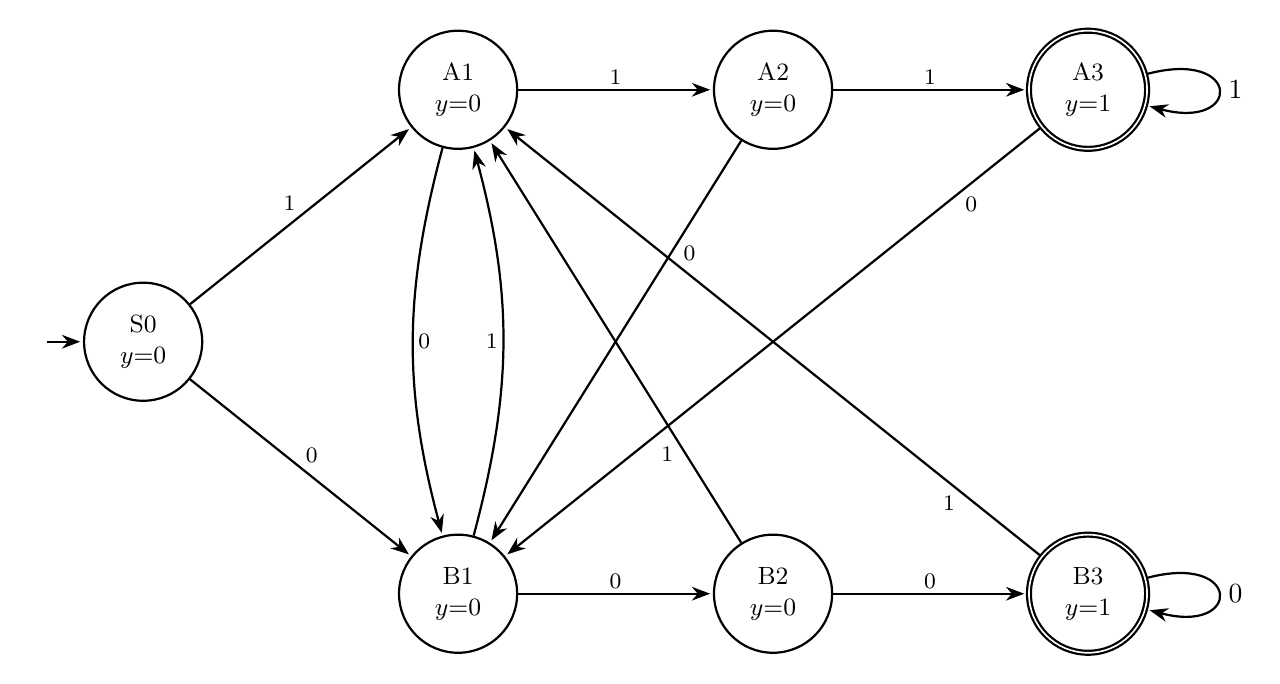
\begin{tikzpicture}[>=Stealth, shorten >=1pt, auto, initial text=, on grid,
  every state/.style={circle,draw,thick,minimum size=1.5cm,inner sep=1pt,font=\small,align=center},
  accepting/.style={accepting by double, accepting distance=2.2pt},
  every edge/.style={draw,thick,->},
  lbl/.style={midway,fill=white,inner sep=1.5pt,font=\footnotesize}]
\node[state,initial] (S0) at (0,0) {S0\\$y{=}0$};
\node[state] (A1) at (4,3.2) {A1\\$y{=}0$};
\node[state] (A2) at (8,3.2) {A2\\$y{=}0$};
\node[state,accepting] (A3) at (12,3.2) {A3\\$y{=}1$};
\node[state] (B1) at (4,-3.2) {B1\\$y{=}0$};
\node[state] (B2) at (8,-3.2) {B2\\$y{=}0$};
\node[state,accepting] (B3) at (12,-3.2) {B3\\$y{=}1$};
\path (S0) edge node[lbl]{1} (A1)
      (S0) edge node[lbl]{0} (B1)
      (A1) edge node[lbl]{1} (A2)
      (A2) edge node[lbl]{1} (A3)
      (A3) edge[loop right] node{1} (A3)
      (A1) edge[bend right=15] node[lbl]{0} (B1)
      (B1) edge[bend right=15] node[lbl]{1} (A1)
      (A2) edge node[lbl,pos=0.25]{0} (B1)
      (A3) edge node[lbl,pos=0.15]{0} (B1)
      (B1) edge node[lbl]{0} (B2)
      (B2) edge node[lbl]{0} (B3)
      (B3) edge[loop right] node{0} (B3)
      (B2) edge node[lbl,pos=0.25]{1} (A1)
      (B3) edge node[lbl,pos=0.15]{1} (A1);
\end{tikzpicture}
\end{document}
